%!TEX root = ../../thesis.tex
\section{Soft robots: what are they?}
\label{sec:intro:history}
Biological systems have long been a source of inspiration for roboticists seeking to create machines with astonishing resilience and capabilities. While humans can effortlessly interact with a wide variety of objects, conventional rigid robots require precise knowledge of an object's weight, shape, and orientation to safely and reliably interact with it. The field of soft robotics has emerged as a new discipline that incorporates methodologies commonly found in nature. Soft robots are constructed from highly compliant materials, and the term "\emph{soft}" is used in contrast to rigid robots, but also refers to the flexible, compressible, and environmentally robust properties associated with soft materials. To achieve bio-like performance in modern machines, researchers believe that the general lack of material diversity in robotics may be the missing piece of the puzzle.

In engineering, a common way to convey a measure of elasticity is the Young's modulus. While limited to homogeneous materials subject to small deformations, it can still be applied to classify rigidity in robotics. To assist the reader, we have included a spectrum of different materials in Figure \ref{fig:1:1}. A careful observation of this spectrum reveals that biological organisms are primarily composed of low-modulus materials (ranging from $10^4$ to $10^7$ \si{Pa}), such as muscle and skin tissue, with rigid materials (such as bone) being much less prevalent. In contrast, conventional robotics predominantly rely on hard materials such as metals and hard plastics. Furthermore, it is worth noting that materials which undergo repeated deformation during motion possess correspondingly low elastic moduli, as opposed to rigid materials in classical robotics. The concept of exploring low-elasticity materials, collectively referred to as \emph{"soft materials"}, has fostered a new philosophy in robotics aimed at unifying robots and biology. Although there exist many definitions of soft materials, we propose the following description:
%
\begin{figure}[!t]
    \centering
    %% This file was created by matlab2tikz.
%
%The latest updates can be retrieved from
%  http://www.mathworks.com/matlabcentral/fileexchange/22022-matlab2tikz-matlab2tikz
%where you can also make suggestions and rate matlab2tikz.
%
\definecolor{mycolor1}{rgb}{0.00784,0.74902,0.90588}%
\definecolor{mycolor2}{rgb}{1.00000,0.16078,0.45882}%
%
\begin{tikzpicture}

\begin{axis}[%
width=0.751\textwidth,
height=0.139\textwidth,
at={(0.116\textwidth,0.002\textwidth)},
scale only axis,
xmin=0,
xmax=1,
ymin=0,
ymax=1,
axis line style={draw=none},
ticks=none,
axis x line*=bottom,
axis y line*=left
]
\end{axis}

\begin{axis}[%
width=0.95\textwidth,
height=0.075\textwidth,
at={(0\textwidth,0.077\textwidth)},
scale only axis,
xmin=0,
xmax=1,
xtick={0,0.1,0.2,0.3,0.4,0.5,0.6,0.7,0.8,0.9,1},
xticklabels={\empty},
ymin=0,
ymax=1,
ytick={0,0.5,1},
yticklabels={\empty},
axis line style={draw=none},
ticks=none,
axis x line*=bottom,
axis y line*=left
]
\end{axis}

\begin{axis}[%
width=0.95\textwidth,
height=0.075\textwidth,
at={(0\textwidth,0\textwidth)},
scale only axis,
clip=false,
xmode=log,
xmin=10000,
xmax=1100000000000,
xtick={10000,100000,1000000,10000000,100000000,1000000000,10000000000,100000000000,1000000000000},
xticklabels={{$\text{10}^{\text{4}}$},{$\text{10}^{\text{5}}$},{$\text{10}^{\text{6}}$},{$\text{10}^{\text{7}}$},{$\text{10}^{\text{8}}$},{$\text{10}^{\text{9}}$},{$\text{10}^{\text{10}}$},{$\text{10}^{\text{11}}$},{$\text{10}^{\text{12}}$}},
xminorticks=true,
ymin=-1,
ymax=1,
ytick={\empty},
axis background/.style={fill=white},
xmajorgrids,
xminorgrids,
ymajorgrids
]
\addplot [color=white, forget plot]
  table[row sep=crcr]{%
10000	0\\
12626.0010987486	0\\
15941.59037456	0\\
20127.8537584994	0\\
25413.4303670264	0\\
32086.9999737045	0\\
40513.0496923538	0\\
51151.7809929315	0\\
64584.2443019698	0\\
81544.0739518515	0\\
102957.556731251	0\\
129994.222441324	0\\
164130.719537513	0\\
207231.464521903	0\\
261650.469874882	0\\
330359.912012834	0\\
417112.461205652	0\\
526646.239348428	0\\
664943.599666505	0\\
839557.86199951	0\\
1060025.84880688	0\\
1338388.75317376	0\\
1689849.78681246	0\\
2133604.52650141	0\\
2693889.30959018	0\\
3401304.93827925	0\\
4294487.98878927	0\\
5422221.00650159	0\\
6846096.83857466	0\\
8643882.62059826	0\\
10913767.1465127	0\\
13779723.5983356	0\\
17398280.5293036	0\\
21967070.9079324	0\\
27735626.1419842	0\\
35019004.6143171	0\\
44214999.0737449	0\\
55825862.688627	0\\
70485740.364519	0\\
88995303.5288522	0\\
112365480.013875	0\\
141872667.41166	0\\
179128445.4622	0\\
226167594.922286	0\\
285559230.19901	0\\
360547115.42505	0\\
455226827.550731	0\\
574769442.483536	0\\
725703961.232423	0\\
916273901.188673	0\\
1156887528.31628	0\\
1460686320.36499	0\\
1844262708.58553	0\\
2328566298.4982	0\\
2940048064.33471	0\\
3712105009.06637	0\\
4686904192.31419	0\\
5917685748.18881	0\\
7471670675.86807	0\\
9433732216.29977	0\\
11911031332.8301	0\\
15038869469.5541	0\\
18988078244.6526	0\\
23974349678.0108	0\\
30270016537.6346	0\\
38218926206.3311	0\\
48255220427.4128	0\\
60927046613.6869	0\\
76926495748.7916	0\\
97127401984.7117	0\\
122633068417.756	0\\
154836525658.55	0\\
195496614309.126	0\\
246834046706.865	0\\
311652694492.944	0\\
393492726309.585	0\\
496823959473.439	0\\
627289985819.623	0\\
792016405019.254	0\\
1000000000000	0\\
};

\addplot[area legend, draw=none, fill=mycolor1, fill opacity=0.75, forget plot]
table[row sep=crcr] {%
x	y\\
10000	-1\\
15000	-1\\
15000	1\\
10000	1\\
}--cycle;
\node[right, align=left, rotate=70]
at (axis cs:9775,1.3) {\scriptsize Hydrogel};

\addplot[area legend, draw=none, fill=mycolor1, fill opacity=0.75, forget plot]
table[row sep=crcr] {%
x	y\\
100000	-1\\
770000	-1\\
770000	1\\
100000	1\\
}--cycle;
\node[right, align=left, rotate=70]
at (axis cs:255850,1.3) {\scriptsize Elastomer};

\addplot[area legend, draw=none, fill=mycolor2, fill opacity=0.75, forget plot]
table[row sep=crcr] {%
x	y\\
20500	-1\\
27500	-1\\
27500	1\\
20500	1\\
}--cycle;
\node[right, align=left, rotate=70]
at (axis cs:19210,1.3) {\scriptsize Skeletal muscle};

\addplot[area legend, draw=none, fill=mycolor2, fill opacity=0.75, forget plot]
table[row sep=crcr] {%
x	y\\
90000	-1\\
110000	-1\\
110000	1\\
90000	1\\
}--cycle;
\node[right, align=left, rotate=70]
at (axis cs:81600,1.3) {\scriptsize Cardiac muscle};

\addplot[area legend, draw=none, fill=mycolor2, fill opacity=0.75, forget plot]
table[row sep=crcr] {%
x	y\\
1258925.41179417	-1\\
1995262.31496888	-1\\
1995262.31496888	1\\
1258925.41179417	1\\
}--cycle;
\node[right, align=left, rotate=70]
at (axis cs:1257852.51,1.3) {\scriptsize Artery};

\addplot[area legend, draw=none, fill=mycolor1, fill opacity=0.75, forget plot]
table[row sep=crcr] {%
x	y\\
31622776.6016838	-1\\
63095734.4480193	-1\\
63095734.4480193	1\\
31622776.6016838	1\\
}--cycle;
\node[right, align=left, rotate=70]
at (axis cs:34904964.362,1.3) {\scriptsize Rubber};

\addplot[area legend, draw=none, fill=mycolor2, fill opacity=0.75, forget plot]
table[row sep=crcr] {%
x	y\\
14000000000	-1\\
16000000000	-1\\
16000000000	1\\
14000000000	1\\
}--cycle;
\node[right, align=left, rotate=70]
at (axis cs:12410000000,1.3) {\scriptsize Bone};

\addplot[area legend, draw=none, fill=mycolor1, fill opacity=0.75, forget plot]
table[row sep=crcr] {%
x	y\\
60000000000	-1\\
66000000000	-1\\
66000000000	1\\
60000000000	1\\
}--cycle;
\node[right, align=left, rotate=70]
at (axis cs:52530000000,1.3) {\scriptsize Aluminium};

\addplot[area legend, draw=none, fill=mycolor1, fill opacity=0.75, forget plot]
table[row sep=crcr] {%
x	y\\
3200000000	-1\\
4000000000	-1\\
4000000000	1\\
3200000000	1\\
}--cycle;
\node[right, align=left, rotate=70]
at (axis cs:2924000000,1.3) {\scriptsize Nylon};

\addplot[area legend, draw=none, fill=mycolor1, fill opacity=0.75, forget plot]
table[row sep=crcr] {%
x	y\\
800000000	-1\\
3000000000	-1\\
3000000000	1\\
800000000	1\\
}--cycle;
\node[right, align=left, rotate=70]
at (axis cs:1241000000,1.3) {\scriptsize Epoxy};

\addplot[area legend, draw=none, fill=mycolor2, fill opacity=0.75, forget plot]
table[row sep=crcr] {%
x	y\\
10000000	-1\\
12000000	-1\\
12000000	1\\
10000000	1\\
}--cycle;
\node[right, align=left, rotate=70]
at (axis cs:9010000,1.3) {\scriptsize Skin};

\addplot[area legend, draw=none, fill=mycolor2, fill opacity=0.75, forget plot]
table[row sep=crcr] {%
x	y\\
8000000000	-1\\
9300000000	-1\\
9300000000	1\\
8000000000	1\\
}--cycle;
\node[right, align=left, rotate=70]
at (axis cs:7131500000,1.3) {\scriptsize Wood};

\addplot[area legend, draw=none, fill=mycolor2, fill opacity=0.75, forget plot]
table[row sep=crcr] {%
x	y\\
89000000000	-1\\
99000000000	-1\\
99000000000	1\\
89000000000	1\\
}--cycle;
\node[right, align=left, rotate=70]
at (axis cs:78200000000,1.3) {\scriptsize Tooth enamel};

\addplot[area legend, draw=none, fill=mycolor1, fill opacity=0.75, forget plot]
table[row sep=crcr] {%
x	y\\
1020000000000	-1\\
1100000000000	-1\\
1100000000000	1\\
1020000000000	1\\
}--cycle;
\node[right, align=left, rotate=70]
at (axis cs:887400000000,1.3) {\scriptsize Diamond};

\addplot[area legend, draw=none, fill=mycolor1, fill opacity=0.75, forget plot]
table[row sep=crcr] {%
x	y\\
190000000000	-1\\
200000000000	-1\\
200000000000	1\\
190000000000	1\\
}--cycle;
\node[right, align=left, rotate=70]
at (axis cs:164050000000,1.3) {\scriptsize Steel};
\node[right, align=left]
at (axis cs:200000000,0.1) {\scriptsize soft};
\node[right, align=left]
at (axis cs:900000000,0.1) {\scriptsize rigid};
\end{axis}

\begin{axis}[%
width=0.969\textwidth,
height=0.171\textwidth,
at={(-0.01\textwidth,-0.017\textwidth)},
scale only axis,
xmin=0,
xmax=1,
ymin=0,
ymax=1,
axis line style={draw=none},
ticks=none,
axis x line*=bottom,
axis y line*=left
]
\draw[-{Stealth}, color=black] (axis cs:0.59,0.2) -- (axis cs:0.15,0.2);
\draw[-{Stealth}, color=black] (axis cs:0.61,0.2) -- (axis cs:0.9,0.2);
\end{axis}
\end{tikzpicture}%
    %\include{./pdf/thesis-figure-1-0.pdf}
    %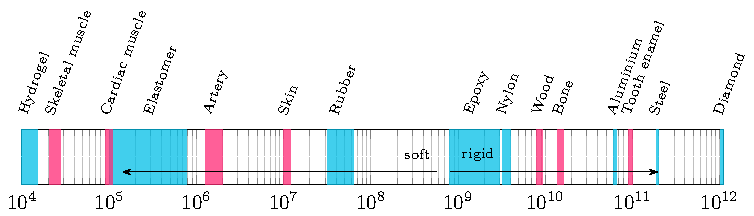
\includepdf[pages=-]{./pdf/thesis-figure-1-0.pdf}
    \includegraphics*[width=\textwidth]{./pdf/thesis-figure-1-0.pdf}
    \caption{\small Young's modulus spectrum in (\si{Pa}) of rigid and soft materials, where (\ldata{Matlab8}) are the organic (\ie, biological) materials and (\ldata{Matlab7}) inorganic materials. Modulus scale is adopted from the work of Rus et al. \cite{Rus2015}.\label{fig:1:1}}
    \vspace{-4mm}
\end{figure}
%
\terminology{\textbf{Soft materials} are homogeneous materials with a Young's modulus, often referred to as the elasticity modulus, that is typically less than or equal to $10^9$ \si{\pascal}. The term \textbf{softness} or \textbf{soft} refers to a collection of mechanical properties that are typically attributed to materials within this spectrum$^1$.}{}\
%
\blfootnote{$^1$It is important to note that the terms "soft" and "flexible" do not hold identical meanings as per the aforementioned definition. For example, slender metal rods are classified as flexible but not soft as the Young's modulus is not within the prespecified range.}
%
Now, despite the fact that the words \emph{"soft"} and \emph{"robotics"} have clear definitions independently, the collocation of the two has sparked many new ideas and perspectives within the robotics community for the past two decades. Figure \ref{fig:C0:softrobotexamples} highlights a few of these soft robots that are inspired by various biological creatures. Throughout its young academic life, several definitions have been coined. Initially, soft robotics referred to robots with variable joint stiffness \cite{AlbuSchaffer2004} or artificial compliance achieved through control \cite{AlbuSchaffer2011}. The term was also used to underline the shift from rigid-linked robots to \textit{"bio-inspired continuum robots are inherently compliant and that exhibit large strains in normal operations"} \cite{Trivedi2008}. Paraphrasing the work of Robison et al. \cite{Robinson1999}: \textit{"soft robotic manipulators are continuum robots made of soft materials that undergo continuous elastic deformation and produce motion through the generation of a smooth backbone curve"}. Alternatively, a broader definition was coined in a review by Kim et al. \cite{Kim2013} simply referring to soft-bodied robots as \textit{"an analogy to soft-bodied animals"}. A concise definition was proposed by Laschi et al. \cite{Laschi2014}, as soft robots being \textit{"any robot built by soft materials"}. Rus et al. \cite{Rus2015} defined soft robots in terms of their structural elasticity: \textit{"Systems that are capable of autonomous behavior, and that are primarily composed of materials with moduli in the range of that of soft biological materials"}.

\par The ongoing debate regarding the precise terminology for soft robotics may never reach a definitive conclusion. It is of utmost importance to establish a uniform vocabulary not just for the sake of this thesis, but also to ensure effective communication across the wider scientific community. Previous definitions have placed great emphasis on the natural motion that arises from soft materials with high similarities to nature. In this thesis, we propose our definition of \textit{"soft robots"} based on the historical development of soft robotics and current scientific trends in literature (discussed in Chapter \ref{chap: history}) with particular focus on design and control. Given the interdisciplinary nature of the field, the terms used in this thesis may differ from those used in existing literature. Throughout the thesis, we will refer to the following definition when discussing "\emph{soft robotics}":
%
\terminology{\textbf{Soft robotics} is a subclass of robotics with purposefully designed compliant actuators embedded into their soft body, that enable control over the soft robot's natural ability to perform bio-inspired morphological behavior.}{}
%
The formulation above, modified from an early definition proposed in \cite{DellaSantina2020Springer}, emphasizes the significance of soft materials in replicating biological motion, also known as "\textit{biomimicry}" or "\textit{biomimetics}". Soft robotics represents the first stepping stone in the pursuit of harmonizing robotics and biological principles. This newly adopted field of soft robotics delves into the use of soft materials not only from a design perspective but also with regard to their implications for control, with the aim of recovering biological morphologies.

\begin{figure}[!t]
    \vspace{-2mm}
    % \ifx\printFigures\undefined
    % \else
    % \hspace{1mm}
    \includegraphics*[width=\textwidth]{./pdf/thesis-figurex-0-0-1.pdf}
    \vspace{-6mm}
    \caption{\small Examples of soft robotic systems that draw inspiration from nature. (a) Festo's Bionic arm inspired by the elephant's trunk but with octopus-inspired gripper \cite{Grzesiak2011}. (b)  Vacuum-driven origami-inspired artificial muscles by Li et al. \cite{Li2017Dec}. Vine-inspired inspection soft robot by Hawkes et al. \cite{Hawkes2017}. Soft robotic fish by Katzschmann et al. \cite{Katzschmann2018} composed of fluid-driven soft actuators \cite{Marchese2014}.
    \label{fig:C0:softrobotexamples}}
    \vspace{-2mm}
  \end{figure}

%In this section, we will present a short historical overview of soft robotics. Hereby showing that the current trends of bio-mimicry and elasticity in robotics find roots in a periods way before the soft robotic boom in the early 2010's. To guide the reader, in Figure \ref{fig:C0:timeline}, we provide a graphical, historic overview of soft robotic systems from 1960 to 2022. We will discuss the inception of soft actuation, early soft robotic designs, and modeling and control strategies for these continuum robotics.